\section{Motivation} \label{sec:motivation}
In this section, we will briefly introduce the widely used 
BFS algorithm and then show the challenge of 
using OpenCL to implement BFS on FPGAs. 

%\subsection{High level FPGA design tools}
%Despite the relatively good performance, 
%the HDL based design typically results in low design productivity, large reuse, 
%portability and maintenance cost as well as ease of use challenge. 
%To address this problem, the FPGA vendors have started 
%to offer high level programming options such as C/C++ and OpenCL, which makes 
%it possible for the designers without much low-level circuit design 
%experiences \cite{nimbix, xilinx-sdaccel, intel-opencl} 
%to program the FPGAs efficiently. In addition, the accelerator 
%described with high level languages preserves many software-like features 
%such as portability, ease of maintenance and use. Considering the  
%continuously growing FPGA resources and stringent time-to-market requirements, 
%the high level FPGA design tools \cite{Nane2016hls-survey} get increasing popularity.
\subsection{OpenCL based BFS on FPGAs}
A typical frontier based BFS algorithm implementation is named as 
level synchronous BFS \cite{attia2014cygraph, betkaoui2012reconfigurable, 
zhang2017boosting}. It has a frontier queue to store the vertices to 
be inspected. Initially, the source vertex is the only vertex in the frontier queue.
By inspecting the frontier vertices, new vertices are traversed and become 
the frontier vertices in next iteration. The graph is iteratively 
processed until the frontier is empty.
Graphs are usually sparse and stored as CSR format. 
CSR includes a row pointer array (RPA) and a column index array (CIA).
RPA contains the starting index of each vertex in CIA array
while CIA consists of the incoming/outgoing neighbors.

%HLS tools greatly alleviate the efforts of building accelerators on FPGAs
%and make FPGAs accessible to designers without much hardware design experiences. 
%This has been well discussed in prior work. Nevertheless, the performance of 
%the resulting accelerators can be far from satisfying especially for 
%irregular applications like BFS. 

To explore the use of OpenCL for BFS acceleration on FPGAs, we deployed 
the reference BFS in Spector \cite{gautier2016spector}, which is an OpenCL 
benchmark targeting FPGAs, on Intel Xeon-FPGA (Harp-v2). In the experiments, 
Intel OpenCL 16.1 is used on Ubuntu 16.04. We measured the BFS performance with 
a set of representative graphs including Youtube (YT), Live Journal(LJ), 
Pokec(PK), and two R-MAT graphs(R19 and R21). Details about the graph 
benchmark can be found in Table \ref{tab:graph} in the experiment section. 
The achieved performance on YT and R19 is 12 and 64 Million Traverse 
Per Second (MTEPS) respectively. It is far from ideal 
compared to the state-of-art handcrafted designs on FPGAs \cite{betkaoui2012reconfigurable}, 
\cite{attia2014cygraph}, \cite{zhang2017boosting}, \cite{nurvitadhi2014graphgen},
\cite{dai2016fpgp}, the performance of which is usually higher 
than 100 MTEPS. The execution gets stuck on the rest of the graphs. 
We failed to fix the bug without changing the kernel 
implementation approach i.e. NDRange kernel \cite{intelOpenCL} 
after quite some efforts. 

%\begin{table}
%    \centering
%	\caption{Open sourced OpenCL BFS on FPGAs}
%  \label{tab:spector-bfs}
%  \begin{tabular}{cccccc}
%    \toprule
%      Benchmark & YT & LJ & PK & R19 & R21 \\
%    \midrule
%	BFS in Spector(MTEPS) & 12 & - & - & 64 & -\\
%	Modified BFS(MTEPS) & 18 & 58 & 57 & 57 & 60 \\
%  \bottomrule
%\end{tabular}
%\vspace{-1em}
%\end{table}

%The BFS implementation in Spector is supposed to be independent with the 
%input graph size, as there are no graph specific parameters in the OpenCL 
%code. Nevertheless, 

The experience indicates that OpenCL based design optimization is highly 
demanded before the BFS implementation can achieve competitive performance. 
In addition, we notice that it is rather challenging 
to optimize OpenCL code especially for OpenCL developers even with OpenCL programming experiences in CPU/GPU as many hardware details 
are hidden behind the compiler and it is difficult
to understand the relation between the OpenCL code and the resulting hardware behaviors. 
Therefore, we argue that having the experienced designers to build the high performance 
OpenCL BFS and offer it as an easy-to-use primitive or library can be a promising 
solution to the above problem.
 
%accelerator using HLS tools remains a challenging task and will be even more difficult for 
%designers without much hardware knowledge. Meanwhile, we also notice that the benefits of 
%the HLS design is also attractive. Despite the difference between Xilinx HLS 
%and Intel OpenCL, porting the design to FPGA devices of different vendors is trivial. 
%
%Therefore, we argue that it is beneficial to have the experienced designers to explore the HLS based 
%application acceleration and provide the HLS solutions to more users without hardware 
%experiences. This motivates us to focus on the high-level BFS accelerator optimization
%and offer open-sourced BFS design with both the near handcrafted performance and 
%the software-like flexibility.

\subsection{Inefficient memory access in BFS}
There are a large amount of memory accesses but little computation in BFS. 
Thus, memory access efficiency is critical to the BFS performance. To gain in-depth 
analysis of the memory access efficiency in BFS with OpenCL, we present two different 
experiments.

In the first experiment, we measured the memory access bandwidth 
of three typical BFS memory access patterns including sequential memory access (SMA), 
dependent random memory access (DRMA) and independent random memory access (IRMA).
Note that DRMA means that the random accesses 
are dependent and they must be handled sequentially while the IRMA 
allows the requests to be processed in parallel. The 
comparison is presented in Figure \ref{fig:avg-mem-lat}. 
It can be found that DRMA has orders of magnitude 
lower bandwidth compared to the other patterns and severely 
underutilizes the hardware memory bandwidth. Thus, we should try 
to avoid memory access in this manner. 

On the other hand, there are many IRMA in BFS.  
However, the compiler can not determine the data dependency during 
compilation and they are taken as dependent. Algorithm \ref{alg:code-seg} 
shows the code segment of BFS that involves the inefficient 
memory accesses. $frontier$ refers to the set of active vertices. 
$v.outgoingNgb$ stands for the set of outgoing neighbors of 
vertex $v$. $l$ is the current level of BFS. $level$ is an 
array of level information of the graph. Typically, the neighbors 
of a vertex are different, so $level$ update in different iterations 
of the inner most loop are independent. But the compiler without 
application specific information does not know that the neighbors 
are different. At compilation, the memory accesses are considered 
as dependent to ensure the correctness in all scenarios, 
which leads to much lower memory bandwidth according to the 
experiment in Figure \ref{fig:avg-mem-lat}.

\vspace{-0.5em}
\begin{algorithm}
\footnotesize
	\caption{Code segment of BFS} \label{alg:code-seg}
	\begin{algorithmic}[2]
		\State ...
		\For{$v \in frontier$}
		\For{$v\_out \in v.outgoingNgb$}
		\If {($level[v\_out] == -1$)}
		\State $level[v\_out] \gets l + 1$
		\EndIf
		\EndFor
		\EndFor
		\State ...
	\end{algorithmic}
\end{algorithm}
\vspace{-0.5em}

To gain insight of the memory accesses in BFS, we analyzed their distribution in the second 
experiment. We extracted the memory access patterns from the trace of 64 non-trivial BFS 
with random starting vertices. When a memory request is less than 16 bytes, we take it as an irregular 
random memory access (IRRMA). According to the experiment result on the five graphs 
in Figure \ref{fig:bfs-mem-dist}, we find that the majority of memory accesses in BFS are irregular, 
though the amount of the memory accesses take up only 15\%-20\% of the total memory accesses. 
Suppose the vertex index is 32-bit, most of the memory accesses such as outgoing neighbor traverse 
in BFS adopt 32-bit data width. As a result, the relatively small data width in combination with the 
irregular memory access patterns incurs rather low memory bandwidth utilization. 
\begin{figure}
	\center{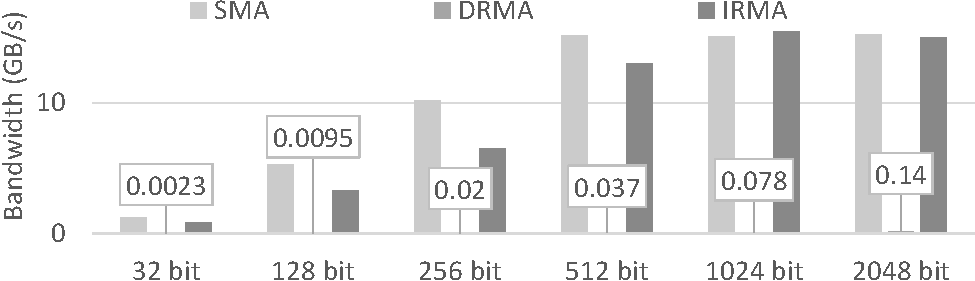
\includegraphics[width=0.75\linewidth]{avg-mem-lat}}
    \caption{Average memory access bandwidth}
\label{fig:avg-mem-lat}
\vspace{-0.5em}
\end{figure}

\begin{figure}
	\center{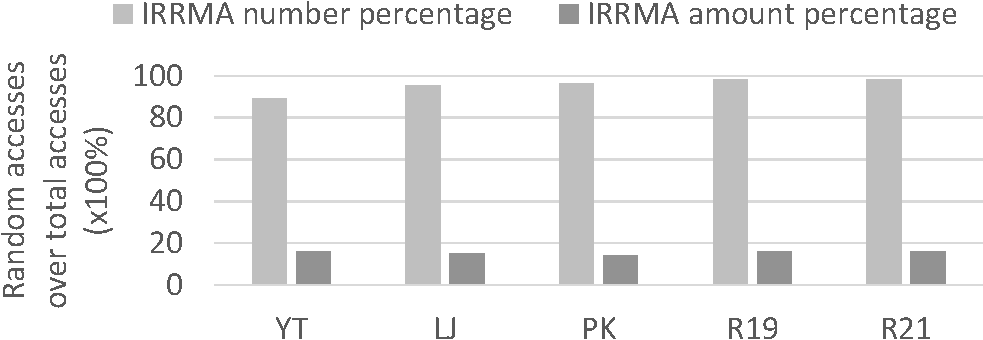
\includegraphics[width=0.75\linewidth]{bfs-mem-dist}}
    \caption{BFS irregular memory access distribution analysis. 'amount' refers to the amount of 
	bytes of memory accesses while 'number' focuses on the number of memory requests.}
\label{fig:bfs-mem-dist}
\vspace{-1em}
\end{figure}

In summary, many random memory accesses in BFS cannot be optimized by the OpenCL compilation. 
Particularly, there are a large number of short and irregular memory
accesses with small data width that underutilize the hardware memory bandwidth. 
In addition, many independent memory accesses in BFS are taken as dependent and the 
false dependency results in rather low memory bandwidth utilization.
These inefficient memory accesses accounts for a large proportion of the total 
memory accesses and BFS is memory intensive. 
%Therefore, memory access optimizations becomes key to improve BFS performance. 
Therefore, memory access optimizations are critical yet challenging to improve BFS 
performance.
